\section{Jumping attempts examples}
In order to test our solutions and ideas, we used recordings of ski jumping attempts from the Four Hills Tournament 2025/2026 (the most recent one) from the two events:
\begin{enumerate}
    \item Obersdorf (GER) - M - Large Hill Qualis - Viessmann FIS Ski Jumping World Cup (28.12.2025)
    \item Garmisch (GER) - M - Large Hill Qualis - Viessmann FIS Ski Jumping World Cup (31.12.2025)
\end{enumerate}

By processing the raw live streams, we extracted \textbf{45 individual jumping clips} from the Oberstdorf event and \textbf{67 clips from Garmisch-Partenkirchen}. All videos were captured at a resolution of 1920$\times$1080 (Full HD). This resulted in a total of 112 unique jumping attempts for analysis.

\section{Jumper detection}
To test detection pipeline, we used the video described above. The detection module, based on a fine-tuned object detector, successfully localized the center of mass. As evidenced by the analysis of sample trajectories, the pipeline integrates a segmentation refinement step and applies Kalman filtering to the raw measurements. Comparing the raw detection output with the filtered states reveals that the Kalman filter effectively mitigates detection noise, resulting in a smooth and continuous flight path. Visual verification confirms that the generated bounding boxes consistently track the jumper's silhouette throughout the flight phase, validating the system's robustness against background clutter and posture changes.

\begin{figure}[H]
    \centering
    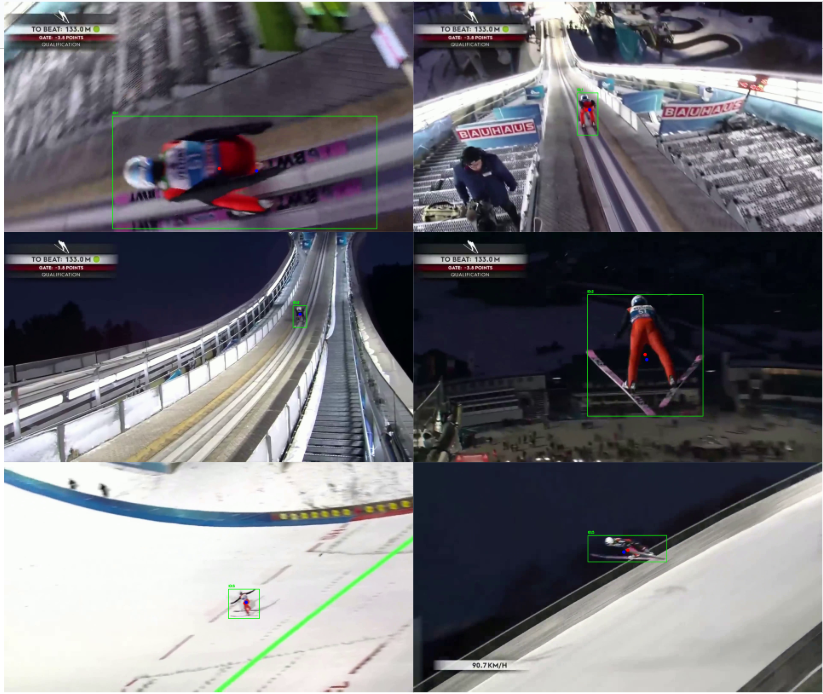
\includegraphics[width=0.9\linewidth]{images/detectionResult.png}
    \caption{6 frames from the video after detection} 
    \label{fig:projection}
\end{figure}

The detection results are satisfactory, having been tested in various videos featuring different events and terrain types. Bounding boxes are tightly fitted without additional margins. Frame loss is rare and easily handled within the pipeline.

Along the output video with drawn bounding box in every frame pipeline produces the \textit{csv} file with the calculated values for each frame in the video. The column names indicate:
\begin{itemize}
    \item \textit{f} - index of the frame,
    \item \textit{id} - track id,
    \item \textit{x1} - x component of the first point of the bounding box,
    \item \textit{y1} - y component of the first point of the bounding box,
    \item \textit{x2} - x component of the second point of the bounding box,
    \item \textit{y2} - y component of the second point of the bounding box,
    \item \textit{mass\_x} - x component of the center of mass,
    \item \textit{mass\_y} - y component of the center of mass,
    \item \textit{kf\_x} - x component of the Kalman filter output,
    \item \textit{kf\_y} - y component of the Kalman filter output,
    \item \textit{score} - score for \texttt{Media pipe} (not used in the final version),
    \item \textit{pose} - 1 if \texttt{Media pipe} used and 0 if not (not used in the final version),
    \item \textit{sam} - 1 if \texttt{SAM3} used and 0 if not.
\end{itemize}

\begin{table}[!ht]
    \centering
    \label{tab:tracking_data}
    \scriptsize
    \begin{tabularx}{\textwidth}{|X|X|X|X|X|X|c|c|c|c|c|c|c|}
    \hline
        \textbf{f} & \textbf{id} & \textbf{x1} & \textbf{y1} & \textbf{x2} & \textbf{y2} & \textbf{mass\_x} & \textbf{mass\_y} & \textbf{kf\_x} & \textbf{kf\_y} & \textbf{score} & \textbf{pose} & \textbf{sam} \\ \hline
        0 & 1 & 804 & 322 & 1332 & 1080 & 1060.00 & 651.00 & 1060.00 & 651.03 & 0.0 & 0 & 1 \\ \hline
        1 & 1 & 806 & 319 & 1338 & 1080 & 1074.00 & 639.00 & 1070.69 & 641.83 & 0.0 & 0 & 1 \\ \hline
        2 & 1 & 810 & 329 & 1354 & 1079 & 1079.00 & 660.00 & 1078.76 & 653.67 & 0.0 & 0 & 1 \\ \hline
        3 & 1 & 812 & 325 & 1373 & 1079 & 1128.00 & 655.00 & 1114.05 & 655.79 & 0.0 & 0 & 1 \\ \hline
        4 & 1 & 813 & 314 & 1396 & 1079 & 1134.00 & 642.00 & 1133.71 & 648.98 & 0.0 & 0 & 1 \\ \hline
        5 & 1 & 822 & 310 & 1416 & 1079 & 1142.00 & 612.00 & 1147.34 & 629.68 & 0.0 & 0 & 1 \\ \hline
        6 & 1 & 825 & 309 & 1421 & 1079 & 1159.00 & 624.00 & 1162.27 & 624.07 & 0.0 & 0 & 1 \\ \hline
        7 & 1 & 830 & 301 & 1426 & 1079 & 1123.00 & 619.00 & 1155.43 & 618.72 & 0.0 & 0 & 1 \\ \hline
        8 & 1 & 817 & 293 & 1441 & 1079 & 1134.00 & 668.00 & 1154.23 & 634.72 & 0.0 & 0 & 1 \\ \hline
        9 & 1 & 810 & 297 & 1459 & 1079 & 1152.00 & 614.00 & 1159.25 & 626.35 & 0.0 & 0 & 1 \\ \hline
        10 & 1 & 823 & 310 & 1474 & 1079 & 1168.00 & 676.00 & 1167.79 & 642.06 & 0.0 & 0 & 1 \\ \hline
        \dots & \dots & \dots & \dots & \dots & \dots & \dots & \dots & \dots & \dots & \dots & \dots & \dots \\ \hline
        171 & 2 & 712 & 337 & 1053 & 761 & 874.00 & 499.00 & 778.93 & 505.42 & 0.0 & 0 & 1 \\ \hline
        172 & 2 & 772 & 313 & 1084 & 754 & 903.00 & 491.00 & 860.23 & 491.81 & 0.0 & 0 & 1 \\ \hline
        173 & 2 & 809 & 289 & 1097 & 765 & 921.00 & 487.00 & 924.25 & 481.15 & 0.0 & 0 & 1 \\ \hline
        \dots & \dots & \dots & \dots & \dots & \dots & \dots & \dots & \dots & \dots & \dots & \dots & \dots \\ \hline
        330 & 6 & 1057 & 591 & 1202 & 729 & 1147.00 & 651.00 & 1150.27 & 653.52 & 0.0 & 0 & 1 \\ \hline
        331 & 6 & 1053 & 596 & 1198 & 734 & 1130.00 & 662.00 & 1136.18 & 658.48 & 0.0 & 0 & 1 \\ \hline
        332 & 6 & 1042 & 600 & 1182 & 739 & 1118.00 & 670.00 & 1122.38 & 664.59 & 0.0 & 0 & 1 \\ \hline
    \end{tabularx}
    \caption{Example of trajectory calculated values}
\end{table}

\section{}